\section{Ejemplos}
\frame{\sectionpage}

\begin{frame}{Ejemplo 1 (Clase 6 de junio)}
    \usetikzlibrary{arrows,shapes}
    
    \pgfdeclarelayer{background}
    \pgfsetlayers{background,main}
    
    \tikzstyle{vertex}=[circle,fill=black,minimum size=20pt,inner sep=0pt]
    \tikzstyle{selected vertex} = [vertex, fill=red]
    \tikzstyle{edge} = [draw,thick,-]
    \tikzstyle{weight} = [font=\small, color=yellow]
    \tikzstyle{selected edge} = [draw,line width=5pt,-,red!50]
    \tikzstyle{ignored edge} = [draw,line width=5pt,-,black!20]

    \begin{figure}
        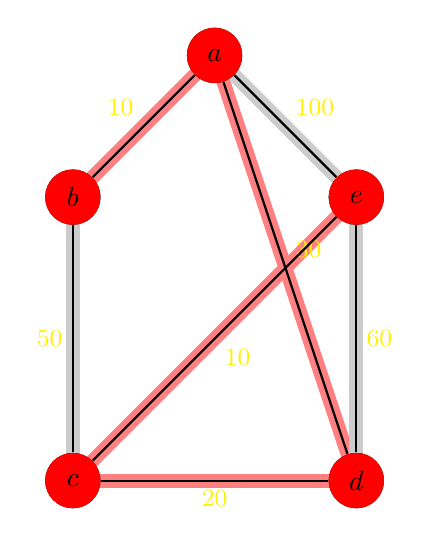
\begin{tikzpicture}[scale=1.8, auto,swap]
            % Draw a 7,11 network
            % First we draw the vertices
            \foreach \pos/\name in {{(0,2)/a}, {(-1,1)/b}, {(-1,-1)/c},
                                    {(1,-1)/d}, {(1,1)/e}}
                \node[vertex] (\name) at \pos {$\name$};
            % Connect vertices with edges and draw weights
            \foreach \source/ \dest /\weight in {a/b/10, b/c/50, e/a/100, d/a/30, c/e/10, c/d/20, d/e/60}
                \path[edge] (\source) -- node[weight] {$\weight$} (\dest);
            % Start animating the vertex and edge selection. 
            \foreach \vertex / \fr in {a/1,b/2,c/3,e/4,d/5}
                \path<\fr-> node[selected vertex] at (\vertex) {$\vertex$};
            % For convenience we use a background layer to highlight edges
            % This way we don't have to worry about the highlighting covering
            % weight labels. 
            \begin{pgfonlayer}{background}
                \pause
                \foreach \source / \dest in {a/b,b/a,c/e,c/d,a/d}
                    \path<+->[selected edge] (\source.center) -- (\dest.center);
                \foreach \source / \dest / \fr in {b/c/7, d/e/8, e/a/9}
                    \path<\fr->[ignored edge] (\source.center) -- (\dest.center);
            \end{pgfonlayer}
        \end{tikzpicture}
    \end{figure}
\end{frame}

\begin{frame}{Resultado Ejemplo 1}
    \usetikzlibrary{arrows,shapes}
    
    \pgfdeclarelayer{background}
    \pgfsetlayers{background,main}
    
    \tikzstyle{vertex}=[circle,fill=black,minimum size=20pt,inner sep=0pt]
    \tikzstyle{selected vertex} = [vertex, fill=red]
    \tikzstyle{edge} = [draw,thick,-]
    \tikzstyle{weight} = [font=\small, color=yellow]
    \tikzstyle{selected edge} = [draw,line width=5pt,-,red!50]
    \tikzstyle{ignored edge} = [draw,line width=5pt,-,black!20]
    
    \begin{figure}
        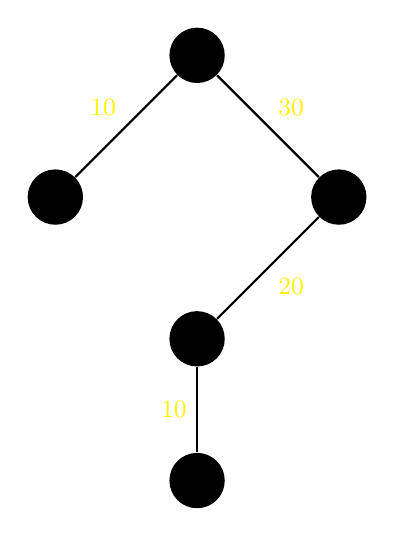
\begin{tikzpicture}[scale=1.8, auto, swap]
            \foreach \pos/\name in {{(0,2)/a}, {(-1,1)/b}, {(0,0)/c},
                                    {(1,1)/d}, {(0,-1)/e}}
                \node[vertex] (\name) at \pos {$\name$};
            \foreach \source/ \dest /\weight in {a/b/10, d/a/30, c/e/10, c/d/20}
                \path[edge] (\source) -- node[weight] {$\weight$} (\dest);
        \end{tikzpicture}
    \end{figure}

    Peso del árbol: 70
\end{frame}

\begin{frame}{Ejemplo 2 (Ejercicio 6, Práctica Parcial 2)}
    \usetikzlibrary{arrows,shapes}
    
    \pgfdeclarelayer{background}
    \pgfsetlayers{background,main}
    
    \tikzstyle{vertex}=[circle,fill=black,minimum size=20pt,inner sep=0pt]
    \tikzstyle{selected vertex} = [vertex, fill=red]
    \tikzstyle{edge} = [draw,thick,-]
    \tikzstyle{weight} = [font=\small, color=yellow]
    \tikzstyle{selected edge} = [draw,line width=5pt,-,red!50]
    \tikzstyle{ignored edge} = [draw,line width=5pt,-,black!20]

    \begin{figure}
        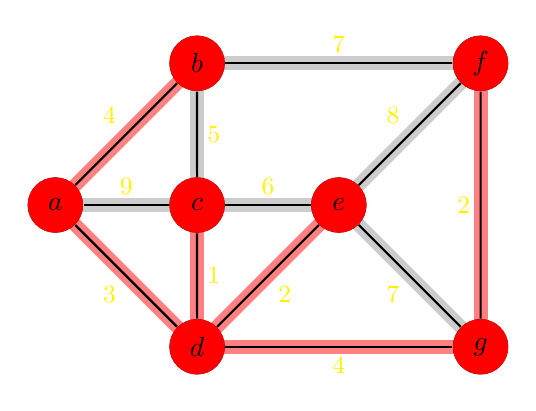
\begin{tikzpicture}[scale=1.8, auto,swap]
            % Draw a 7,11 network
            % First we draw the vertices
            \foreach \pos/\name in {{(0,0)/a}, {(1,1)/b}, {(1,0)/c},
                                    {(1,-1)/d}, {(2,0)/e}, {(3,1)/f}, {(3,-1)/g}}
                \node[vertex] (\name) at \pos {$\name$};
            % Connect vertices with edges and draw weights
            \foreach \source/ \dest /\weight in {b/a/4, c/a/9, a/d/3, c/b/5, f/b/7, d/c/1, e/c/6, d/e/2, d/g/4, f/e/8, e/g/7, f/g/2}
                \path[edge] (\source) -- node[weight] {$\weight$} (\dest);
            % Start animating the vertex and edge selection. 
            \foreach \vertex / \fr in {c/1, d/2, e/3, f/4, g/5, a/6, b/7}
                \path<\fr-> node[selected vertex] at (\vertex) {$\vertex$};
            % For convenience we use a background layer to highlight edges
            % This way we don't have to worry about the highlighting covering
            % weight labels. 
            \begin{pgfonlayer}{background}
                \pause
                \foreach \source / \dest in {c/d, d/e, e/d, f/g, a/d, a/b, d/g}
                    \path<+->[selected edge] (\source.center) -- (\dest.center);
                \foreach \source / \dest / \fr in {b/c/8, c/e/9, b/f/10, e/g/10, e/f/11, a/c/12}
                    \path<\fr->[ignored edge] (\source.center) -- (\dest.center);
            \end{pgfonlayer}
        \end{tikzpicture}
    \end{figure}
\end{frame}

\begin{frame}{Resultado Ejemplo 2}
    \usetikzlibrary{arrows,shapes}
    
    \pgfdeclarelayer{background}
    \pgfsetlayers{background,main}
    
    \tikzstyle{vertex}=[circle,fill=black,minimum size=20pt,inner sep=0pt]
    \tikzstyle{selected vertex} = [vertex, fill=red]
    \tikzstyle{edge} = [draw,thick,-]
    \tikzstyle{weight} = [font=\small, color=yellow]
    \tikzstyle{selected edge} = [draw,line width=5pt,-,red!50]
    \tikzstyle{ignored edge} = [draw,line width=5pt,-,black!20]
    
    \begin{figure}
        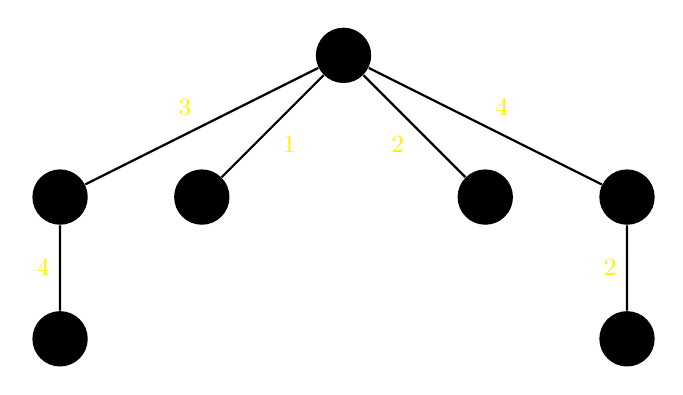
\begin{tikzpicture}[scale=1.8, auto, swap]
            \foreach \pos/\name in {{(0,2)/d}, {(-2,1)/a}, {(-1,1)/c},
                                    {(1,1)/e}, {(2,1)/g}, {(-2,0)/b}, {(2,0)/f}}
                \node[vertex] (\name) at \pos {$\name$};
            \foreach \source/ \dest /\weight in {d/a/3, c/d/1, d/e/2, g/d/4, a/b/4, g/f/2}
                \path[edge] (\source) -- node[weight] {$\weight$} (\dest);
        \end{tikzpicture}
    \end{figure}

    Peso del árbol: 16
\end{frame}